\section{Thermal states and detailed balance}\label{sec:2.5}

At \SI{300}{K} each optical phonon mode of silicon at the zone center, at \SI{64}{meV}, holds on average 0.09 quanta; at the \SI{4}{K} of a liquid-helium cryostat it holds $10^{-81}$. A crystal at a finite temperature is not in an eigenstate of its Hamiltonian, as the rates of \cref{sec:2.1,sec:2.2} assumed, but in a statistical mixture of them, and an excited component of the mixture can give its energy to the dark matter. This is the negative $\omega$ that \cref{sec:1.3} allowed. At zero temperature the same occupation numbers produce the filled Fermi sea of a free electron gas, whose Fermi momentum and density of states \cref{chap:4} uses throughout. We follow Refs.~\cite{landau1980statistical} and \cite[Chap.~1]{bruus2004many} for the ensembles and Ref.~\cite[Chap.~2]{ashcroft1976solid} for the free electron gas.

\subsection{Gibbs state}

A mixture that holds the eigenstate $|i\rangle$ with probability $p_i$ is described by the density matrix
\begin{equation}
  \op{\varrho} = \sum_i p_i\,|i\rangle\langle i|, \qquad \langle\op{A}\rangle = \Tr\bigl(\op{\varrho}\,\op{A}\bigr) = \sum_i p_i\,\langle i|\op{A}|i\rangle ,
  \label{eq:2.5-rho}
\end{equation}
with $\sum_ip_i = 1$; the thermal average $\langle\op{A}\rangle$ is the quantum expectation value averaged over the mixture. A target in equilibrium with a bath at temperature $T$ has the Gibbs weights
\begin{equation}
  p_i = \frac{\ee^{-\beta E_i}}{\mathcal{Z}}, \qquad \mathcal{Z} = \sum_i\ee^{-\beta E_i} = \Tr\,\ee^{-\beta H}, \qquad \beta = \frac{1}{T},
  \label{eq:2.5-gibbs}
\end{equation}
so that $\op{\varrho} = \ee^{-\beta H}/\mathcal{Z}$, with $\mathcal{Z}$ the partition function. In natural units temperature is an energy, $\SI{1}{K} = \SI{86.17}{\micro eV}$, and a detector at \SI{10}{mK} has $T = \SI{0.86}{\micro eV}$.

Since the Gibbs state is a function of $H$, it commutes with $H$, and its time evolution $\op{\varrho}(t) = \ee^{-\ii Ht}\op{\varrho}\,\ee^{\ii Ht}$ leaves it unchanged: it is a stationary state, and every thermal average is independent of time. A correlation $\langle\op{A}(t)\op{B}(t')\rangle$ of Heisenberg operators $\op{A}(t) = \ee^{\ii Ht}\op{A}\,\ee^{-\ii Ht}$ depends only on $t - t'$, which is what makes its Fourier transform in time a function of one frequency (\cref{sec:4.1}). Note that stationarity does not need the Gibbs form; any $\op{\varrho}$ diagonal in the energy basis has it. Thermal equilibrium fixes the weights.

Particles can also be exchanged with a reservoir, or we may prefer to fix their mean number instead of the exact one. The grand-canonical state then replaces $H$ by $H - \mu_{\mathrm{ch}}\op{N}$, with $\op{N}$ the particle-number operator and $\mu_{\mathrm{ch}}$ the chemical potential:
\begin{equation}
  \op{\varrho} = \frac{\ee^{-\beta(H - \mu_{\mathrm{ch}}\op{N})}}{\mathcal{Z}}, \qquad p_i = \frac{\ee^{-\beta(E_i - \mu_{\mathrm{ch}}N_i)}}{\mathcal{Z}} .
  \label{eq:2.5-grand}
\end{equation}
The value of $\mu_{\mathrm{ch}}$ is fixed by $\langle\op{N}\rangle = N$. A detector holds a fixed number of electrons, and the canonical state is the physical one. However, the two ensembles differ in a macroscopic body by fluctuations of relative size $N^{-1/2}$, and the grand-canonical state is much easier to use, since for independent particles it factorizes into one factor per single-particle state (\cref{eq:2.5-nF} below).

\subsection{Thermal golden rule}

The probability of finding the system in $|f\rangle$ at time $t$ is linear in the initial density matrix. With $U(t)$ the evolution operator,
\begin{equation*}
  \langle f|U(t)\,\op{\varrho}\,U(t)^\dagger|f\rangle = \sum_ip_i\,|\langle f|U(t)|i\rangle|^2 = \sum_ip_i\,P_{i\to f}(t) .
\end{equation*}
Different initial states do not interfere, because $\op{\varrho}$ has no off-diagonal elements between them. Each $P_{i\to f}$ grows at its golden-rule rate (\cref{eq:2.1-golden}), and the rate out of the thermal state is the weighted sum
\begin{equation}
  \varGamma = \sum_ip_i\sum_f\varGamma_{i\to f} .
  \label{eq:2.5-thermalrate}
\end{equation}
For dark-matter scattering the initial state is the product of the thermal target and a dark-matter plane wave of momentum $\vect{p}$, and the final state has the target in $|f\rangle$ and the dark matter at $\vect{p} - \vect{q}$. The interaction between these two dark-matter states is $\tilde V(\vect{q})\,n_e(\vect{q})/\Vol$ (\cref{eq:2.3-nq}), and energy conservation, with the dark-matter energies written out, is $\delta(\omega_{\vect{q}} - E_f + E_i)$, where $\omega_{\vect{q}}$ is the energy lost by the dark matter (\cref{eq:1.3-omegaq}). Summing \cref{eq:2.5-thermalrate} over the final momenta,
\begin{equation*}
  \varGamma = \sum_{\vect{q}}\frac{2\pi}{\Vol^2}\,|\tilde V(\vect{q})|^2\,\mathcal{S}_{n_e(\vect{q})}(\omega_{\vect{q}}),
\end{equation*}
where all the target physics sits in the transition sum of an operator $\op{O}$,
\begin{equation}
  \mathcal{S}_O(\omega) = \sum_{i,f}p_i\,|\langle f|\op{O}|i\rangle|^2\,\delta(\omega - E_f + E_i) .
  \label{eq:2.5-transum}
\end{equation}
It counts the transitions that $\op{O}$ drives from the thermal state, weighted by their probability, at each energy $\omega$ given to the target. The same object is the Fourier transform of a thermal correlation function. Inserting a complete set of states between the operators of $\langle\op{O}^\dagger(t)\op{O}(0)\rangle$, each term oscillates as $\ee^{\ii(E_i - E_f)t}$, and the time integral turns it into a delta function:
\begin{equation}
  \int_{-\infty}^{\infty}\dd t\;\ee^{\ii\omega t}\,\langle\op{O}^\dagger(t)\,\op{O}(0)\rangle = 2\pi\,\mathcal{S}_O(\omega) .
  \label{eq:2.5-corr}
\end{equation}
The rate measures how the fluctuations of $\op{O}$ in the equilibrium state are correlated in time, the viewpoint that \cref{sec:4.2} develops. With \cref{eq:2.1-box} for the sum over $\vect{q}$,
\begin{keyresult}[Thermal golden rule]
\begin{equation}
  \varGamma = \int\frac{\dd^3q}{(2\pi)^3}\,\underbrace{|\tilde V(\vect{q})|^2}_{\text{coupling}}\,\underbrace{S(\vect{q},\omega_{\vect{q}})}_{\text{target}}, \qquad
  S(\vect{q},\omega) = \frac{2\pi}{\Vol}\,\mathcal{S}_{n_e(\vect{q})}(\omega) .
  \label{eq:2.5-golden}
\end{equation}
$\varGamma$ is the scattering rate of one dark-matter particle of momentum $\vect{p}$ in a box of volume $\Vol$ filled by the target, which is in thermal equilibrium at temperature $T$.
\end{keyresult}
The function $S(\vect{q},\omega)$ is the dynamic structure factor of the electron density (\cref{eq:A.7-S})~\cite[Eq.~(4)]{knapen2021dark}; that reference writes the density at $-\vect{k}$ where we write $n_e(\vect{q})$ (\cref{app:A.7}); \cref{sec:4.2} develops it. The volume drops out as it should. The transition sum is extensive, since a target twice as large offers twice as many transitions, and $S$ is intensive. The rate of one dark-matter particle, present with density $1/\Vol$ in a target of volume $\Vol$, is then independent of $\Vol$.

The rate assembled in \cref{sec:1.5} now follows. For a target whose response depends only on $q = |\vect{q}|$, we write $S(q,\omega_{\vect{q}}) = \int\dd\omega\,S(q,\omega)\,\delta(\omega - \omega_{\vect{q}})$. The average of the delta function over the direction of $\vect{q}$ and over the halo is $\eta(\vmin)/2q$ (\cref{sec:1.3}; \cref{eq:2.2-spectrum}), and the measure becomes $\int\dd^3q/(2\pi)^3\,(2q)^{-1} = \int q\,\dd q/(2\pi)^2$. Multiplying by the number density $\rho_\chi/m_\chi$ of dark matter, dividing by the target mass density $\rho_T$ and inserting $|\tilde V|^2 = \pi\sigmae\FDM^2/\mu_{\chi e}^2$ (\cref{eq:1.4-Vsq}) reproduces \cref{eq:1.5-rate} term by term. Unlike the version of \cref{sec:1.5}, the derivation holds at any temperature, with the thermal weights inside $S$, and its integral over $\omega$ runs over negative values too.

\subsection{Detailed balance}

Negative $\omega$ means that the target gives energy to the dark matter. The weight of such transitions is tied to the weight of the reverse ones by relabeling the sum. Write the transition sum of $\op{O}^\dagger$ at $-\omega$ and exchange the names of the summed states $i$ and $f$:
\begin{equation*}
  \mathcal{S}_{O^\dagger}(-\omega) = \sum_{i,f}p_i\,|\langle f|\op{O}^\dagger|i\rangle|^2\,\delta(-\omega - E_f + E_i)
  = \sum_{i,f}p_f\,|\langle i|\op{O}^\dagger|f\rangle|^2\,\delta(\omega - E_f + E_i) .
\end{equation*}
Since $|\langle i|\op{O}^\dagger|f\rangle| = |\langle f|\op{O}|i\rangle|$, the identity of \cref{sec:2.1}, the matrix elements are those of $\mathcal{S}_O(\omega)$. The weights differ: the delta function sets $E_f = E_i + \omega$, where $p_f = p_i\,\ee^{-\beta\omega}$. Hence
\begin{keyresult}[Detailed balance]
\begin{equation}
  \mathcal{S}_{O^\dagger}(-\omega) = \ee^{-\beta\omega}\,\mathcal{S}_O(\omega) .
  \label{eq:2.5-db}
\end{equation}
For the electron density, $n_e(\vect{q})^\dagger = n_e(-\vect{q})$, and $S(-\vect{q},-\omega) = \ee^{-\beta\omega}S(\vect{q},\omega)$. For a target with inversion or time-reversal symmetry, $S(\vect{q},-\omega) = \ee^{-\beta\omega}S(\vect{q},\omega)$. The density form is the diagonal element of \cref{eq:A.7-DB}.
\end{keyresult}
In the grand-canonical state the weights carry $-\mu_{\mathrm{ch}}N$ as well, and the step $p_f = p_i\ee^{-\beta\omega}$ needs $N_f = N_i$. It holds for every operator that conserves particle number, such as $n_e(\vect{q})$; an operator that adds $\Delta N$ particles acquires the factor $\ee^{-\beta(\omega - \mu_{\mathrm{ch}}\Delta N)}$ instead. The symmetric form uses $S(-\vect{q},\omega) = S(\vect{q},\omega)$, which inversion or time reversal guarantees (\cref{app:A.4}); silicon has both.

Detailed balance holds for every target in equilibrium, whatever its interactions, because the argument used only the Gibbs weights. In a two-level system with splitting $\Delta_{\mathrm{tl}}$, driven by a Hermitian $\op{O}$ with matrix element $O_{10} = \langle 1|\op{O}|0\rangle$, the transition sum is
\begin{equation*}
  \mathcal{S}_O(\omega) = |O_{10}|^2\bigl[p_0\,\delta(\omega - \Delta_{\mathrm{tl}}) + p_1\,\delta(\omega + \Delta_{\mathrm{tl}})\bigr], \qquad \frac{p_1}{p_0} = \ee^{-\beta\Delta_{\mathrm{tl}}} .
\end{equation*}
The upward transition, at $\omega = +\Delta_{\mathrm{tl}}$, starts from the ground state; the downward one, at $\omega = -\Delta_{\mathrm{tl}}$, starts from the excited state and carries its population (\cref{fig:2-twolevel}). At $T = \Delta_{\mathrm{tl}}/2$ the weights are 0.881 and 0.119. At $T = 0$ the downward weight vanishes and $\omega \ge 0$. As $T \to \infty$ both tend to $\tfrac12$, but the upward weight never falls below the downward one: a thermal target always absorbs more often than it emits, by the factor $\ee^{\beta\omega}$.

\begin{figure}[tbp]
  \centering
  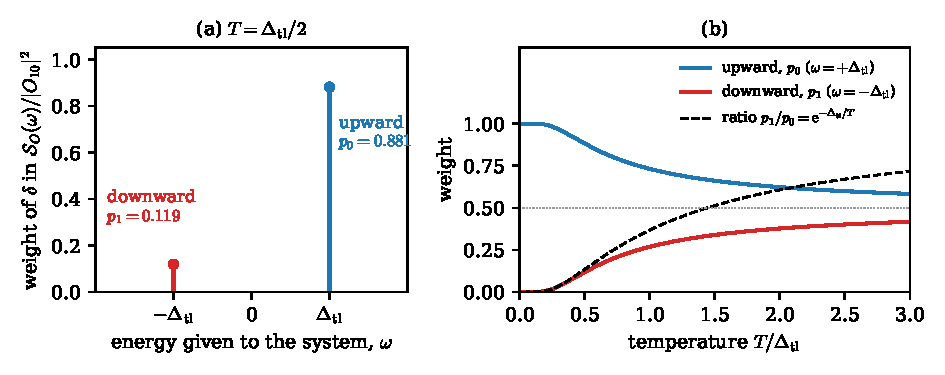
\includegraphics[width=\linewidth]{figures/ch02/fig2_6.pdf}
  \caption{Upward and downward transitions of a two-level system with splitting $\Delta_{\mathrm{tl}}$ in thermal equilibrium at temperature $T$, driven by a Hermitian operator $\op{O}$ with matrix element $O_{10}$. (a) At $T = \Delta_{\mathrm{tl}}/2$ the transition sum $\mathcal{S}_O(\omega)$ consists of two delta functions, drawn as stems with their weights in units of $|O_{10}|^2$. Upward, at energy $\omega = +\Delta_{\mathrm{tl}}$ given to the system, with the ground-state population $p_0 = 0.881$; downward, at $\omega = -\Delta_{\mathrm{tl}}$, with the excited-state population $p_1 = 0.119$. (b) The two weights against $T/\Delta_{\mathrm{tl}}$, and their ratio $p_1/p_0 = \ee^{-\Delta_{\mathrm{tl}}/T}$ (detailed balance). The weights approach $\tfrac12$ (dotted line) from either side as $T$ grows and never cross.}
  \label{fig:2-twolevel}
\end{figure}

The negative-$\omega$ part of the rate is suppressed by the Boltzmann factor of the excitation it removes, $\ee^{-\beta|\omega|}$ relative to the positive-$\omega$ part at the same $|\omega|$. For a \SI{1}{meV} acoustic phonon at \SI{1}{K}, $\beta\omega = 11.6$ and the factor is $9\times10^{-6}$; \cref{app:A.4} gives the case of an electronic gap. Note that such an event deposits no energy in the detector. The target loses energy to the dark matter, and a calorimeter or a charge readout registers nothing. Such transitions nevertheless matter in three places: in the total scattering rate, in the $\omega$ integrals of sum rules (\cref{sec:4.3}), and in the factor $1 - \ee^{-\beta\omega}$ that relates $S$ to the dissipative part of the response, the fluctuation--dissipation theorem (\cref{eq:A.7-FDT}, \cref{sec:4.2}).

\subsection{Occupation of a mode}

The thermal factors $n$ and $n + 1$ of a bosonic mode (\cref{sec:2.3}) follow from the grand-canonical state of independent particles. For $H - \mu_{\mathrm{ch}}\op{N} = \sum_\gamma(E_\gamma - \mu_{\mathrm{ch}})\,c^\dagger_\gamma c_\gamma$ the exponential in \cref{eq:2.5-grand} is a product over single-particle states $\gamma$, and so is $\mathcal{Z}$. Each fermion factor has $n_\gamma = 0$ or $1$, and each boson factor $n_\gamma = 0, 1, 2, \dots$, a geometric series. The mean occupation of one state follows by weighting $n_\gamma$ with its factor:
\begin{equation}
  \langle c^\dagger_\gamma c_\gamma\rangle = \frac{\ee^{-\beta(E_\gamma - \mu_{\mathrm{ch}})}}{1 + \ee^{-\beta(E_\gamma - \mu_{\mathrm{ch}})}} = n_{\mathrm{F}}(E_\gamma - \mu_{\mathrm{ch}}), \qquad
  \langle d^\dagger_\gamma d_\gamma\rangle = \frac{\sum_n n\,\ee^{-\beta nE_\gamma}}{\sum_n\ee^{-\beta nE_\gamma}} = n_{\mathrm{B}}(E_\gamma) ,
  \label{eq:2.5-nF}
\end{equation}
with the Fermi and Bose functions $n_{\mathrm{F}}(x) = (\ee^{\beta x} + 1)^{-1}$ and $n_{\mathrm{B}}(x) = (\ee^{\beta x} - 1)^{-1}$~\cite{landau1980statistical}. A mode with $E_\gamma \ll T$ holds $n_{\mathrm{B}} \approx T/E_\gamma$ quanta, the classical equipartition value, and a mode with $E_\gamma \gg T$ holds $n_{\mathrm{B}} \approx \ee^{-\beta E_\gamma}$. The boson form has no chemical potential. Phonons and magnons are created and destroyed freely, their number is not conserved, and the free energy is at its minimum when $\mu_{\mathrm{ch}} = 0$. The reversed products follow from \cref{eq:2.3-anticomm,eq:2.3-comm}: $\langle c_\gamma c^\dagger_\gamma\rangle = 1 - n_{\mathrm{F}}$, the probability that the state is free to receive an electron, and $\langle d_\gamma d^\dagger_\gamma\rangle = n_{\mathrm{B}} + 1$. Absorbing a boson from a thermal mode has the weight $n_{\mathrm{B}}$ and emitting one has $n_{\mathrm{B}} + 1$, and $(n_{\mathrm{B}} + 1)/n_{\mathrm{B}} = \ee^{\beta E_\gamma}$ is detailed balance for a single mode. Off-diagonal averages $\langle c^\dagger_\gamma c_{\gamma'}\rangle$ with $\gamma \ne \gamma'$ vanish, since $\op{\varrho}$ conserves each occupation.

The fermion factors decide the transition sum of the density for independent electrons. By \cref{eq:2.3-onebody}, $n_e(\vect{q}) = \sum_{\gamma\gamma'}\langle\gamma'|\ee^{\ii\vect{q}\cdot\vect{r}}|\gamma\rangle\,c^\dagger_{\gamma'}c_\gamma$. Acting on an occupation-number state $|i\rangle$, each term with $\gamma' \ne \gamma$ moves one electron and leads to its own final state, and the sum over those final states of $|\langle f|c^\dagger_{\gamma'}c_\gamma|i\rangle|^2$ is $\langle i|c^\dagger_\gamma c_{\gamma'}c^\dagger_{\gamma'}c_\gamma|i\rangle = n_\gamma(1 - n_{\gamma'})$. The terms with $\gamma' = \gamma$ leave the state unchanged and contribute only at $\omega = 0$. The Gibbs state of independent electrons is a product over orbitals, the average of $n_\gamma(1 - n_{\gamma'})$ factorizes, and for $\omega \ne 0$
\begin{equation}
  \mathcal{S}_{n_e(\vect{q})}(\omega) = \sum_{\gamma\ne\gamma'}|\langle\gamma'|\ee^{\ii\vect{q}\cdot\vect{r}}|\gamma\rangle|^2\,n_{\mathrm{F}}(E_\gamma - \mu_{\mathrm{ch}})\bigl[1 - n_{\mathrm{F}}(E_{\gamma'} - \mu_{\mathrm{ch}})\bigr]\,\delta(\omega - E_{\gamma'} + E_\gamma) .
  \label{eq:2.5-indep}
\end{equation}
An electron must be present in $\gamma$, with probability $n_{\mathrm{F}}$, and $\gamma'$ must be free to receive it, with probability $1 - n_{\mathrm{F}}$: this is Pauli blocking at finite temperature. The identity $n_{\mathrm{F}}(E')[1 - n_{\mathrm{F}}(E)] = \ee^{-\beta(E' - E)}\,n_{\mathrm{F}}(E)[1 - n_{\mathrm{F}}(E')]$, with both energies measured from $\mu_{\mathrm{ch}}$, makes \cref{eq:2.5-db} visible term by term. In a semiconductor at $T \ll \Eg$ the factors are one for a filled valence state $\gamma$ and an empty conduction state $\gamma'$ and zero otherwise, and \cref{eq:2.5-indep} becomes a sum over valence-to-conduction transitions of the squared single-particle form factor of \cref{eq:2.3-ph}. With the spin sum supplying the factor 2 of a spin-independent vertex, and written in Bloch states, that sum is the crystal form factor.

\begin{workedexample}{Scattering off a thermal harmonic oscillator}\label{we:2-oscillator}
Let the target be a single mode, $H = \omega_0(d^\dagger d + \tfrac12)$, in equilibrium at temperature $T$, and let the dark matter couple to its displacement, $\op{O} = \lambda_{\mathrm{osc}}(d + d^\dagger)$, with a coupling $\lambda_{\mathrm{osc}}$ that depends on $\vect{q}$. A phonon mode coupled to a nuclear recoil has this form (\cref{sec:5.3}). By \cref{eq:2.3-boson}, $\op{O}$ connects $|n\rangle$ to $|n + 1\rangle$ with the matrix element $\lambda_{\mathrm{osc}}\sqrt{n + 1}$ and to $|n - 1\rangle$ with $\lambda_{\mathrm{osc}}\sqrt{n}$. The transition sum \cref{eq:2.5-transum} is therefore
\begin{equation*}
  \begin{split}
  \mathcal{S}_O(\omega) &= |\lambda_{\mathrm{osc}}|^2\sum_np_n\bigl[(n + 1)\,\delta(\omega - \omega_0) + n\,\delta(\omega + \omega_0)\bigr]\\
  &= |\lambda_{\mathrm{osc}}|^2\bigl[(n_{\mathrm{B}} + 1)\,\delta(\omega - \omega_0) + n_{\mathrm{B}}\,\delta(\omega + \omega_0)\bigr],
  \end{split}
\end{equation*}
with $n_{\mathrm{B}} = n_{\mathrm{B}}(\omega_0) = \sum_np_nn$ by \cref{eq:2.5-nF}. Emission of a quantum, which takes energy from the dark matter, has the weight $n_{\mathrm{B}} + 1$; absorption of a quantum, which gives energy to the dark matter, has the weight $n_{\mathrm{B}}$. At the same $\vect{q}$ their ratio is
\begin{equation*}
  \frac{\mathcal{S}_O(+\omega_0)}{\mathcal{S}_O(-\omega_0)} = \frac{n_{\mathrm{B}} + 1}{n_{\mathrm{B}}} = \ee^{\beta\omega_0},
\end{equation*}
as \cref{eq:2.5-db} requires, since $\op{O}$ is Hermitian. The ratio of the two scattering rates also contains the dark-matter kinematics: the energy-loss rate at fixed $q$ carries $\eta(\vmin(q, +\omega_0))$ and the energy-gain rate $\eta(\vmin(q, -\omega_0))$ (\cref{eq:1.3-vmin}). The minimum velocity for energy gain, $|q/2m_\chi - \omega_0/q|$, vanishes at $q = (2m_\chi\omega_0)^{1/2}$, and gain is kinematically allowed for every dark-matter mass.

For numbers, take the \SI{64}{meV} optical phonon of silicon at the zone center. At \SI{300}{K}, $\beta\omega_0 = 2.48$, $n_{\mathrm{B}} = 0.092$, and the loss-to-gain ratio of the target factors is $\ee^{2.48} = 11.9$. At \SI{4}{K}, $\beta\omega_0 = 186$ and $n_{\mathrm{B}} = 2.3\times10^{-81}$. For a \SI{1}{meV} acoustic phonon, $n_{\mathrm{B}} = 9.1\times10^{-6}$ at \SI{1}{K} and $10^{-252}$ at \SI{20}{mK}, but $1.27$ at \SI{20}{K}, where the ratio is 1.79. A cryogenic detector is in its ground state for every mode above a few tens of \si{\micro eV}, and the ``$+1$'' of spontaneous emission is the whole signal: the dark matter creates a phonon in an empty mode.

The total weight $\int\dd\omega\,\mathcal{S}_O$ and the first moment $\int\dd\omega\,\omega\,\mathcal{S}_O$ respond differently to temperature. The total weight is $\int\dd\omega\,\mathcal{S}_O = |\lambda_{\mathrm{osc}}|^2(2n_{\mathrm{B}} + 1)$, which grows with $T$ because the thermal fluctuations of the displacement grow; at \SI{300}{K} it is 1.18 times the value at $T = 0$ for the optical phonon. The first moment is $\int\dd\omega\,\omega\,\mathcal{S}_O = |\lambda_{\mathrm{osc}}|^2\omega_0[(n_{\mathrm{B}} + 1) - n_{\mathrm{B}}] = |\lambda_{\mathrm{osc}}|^2\omega_0$, independent of $T$, because the thermal populations cancel between emission and absorption. This is the oscillator's version of the f-sum rule (\cref{eq:A.7-fsum}, \cref{sec:4.3}); it requires the negative-$\omega$ weight.
\end{workedexample}

\subsection{Free electron gas at zero temperature}

Jellium with its Coulomb interaction dropped (\cref{we:2-jellium}) is a gas of free electrons, $H = \sum_{\vect{k}s}(k^2/2m_e)\,c^\dagger_{\vect{k}s}c_{\vect{k}s}$, and its occupations are $n_{\mathrm{F}}(k^2/2m_e - \mu_{\mathrm{ch}})$. As $T \to 0$ the Fermi function becomes a step, $n_{\mathrm{F}}(x) \to \Theta(-x)$: every state below $\mu_{\mathrm{ch}}$ is filled and every state above it is empty. The ground state is the Fermi sea, $\prod_{k < k_{\mathrm{F}},\,s}c^\dagger_{\vect{k}s}|0\rangle$, the filled sphere of radius $k_{\mathrm{F}}$ in $\vect{k}$ space, and the chemical potential at $T = 0$ is the Fermi energy $E_{\mathrm{F}} = k_{\mathrm{F}}^2/2m_e$. Counting two spin states and the volume $(2\pi)^3/\Vol$ per wavevector (\cref{eq:2.1-box}), $N_e = 2\Vol(4\pi k_{\mathrm{F}}^3/3)/(2\pi)^3 = Vk_{\mathrm{F}}^3/3\pi^2$. The density of states per spin and per unit volume at energy $E$ is $\mathcal{D}_f(E)/\Vol = m_ek/2\pi^2$, from \cref{eq:2.1-Dfree}, and at the Fermi level it is $\mathcal{N}_{\mathrm{F}}$.
\begin{keyresult}[Free electron gas at $T = 0$]
\begin{equation}
  k_{\mathrm{F}} = (3\pi^2\nd_e)^{1/3}, \qquad E_{\mathrm{F}} = \frac{k_{\mathrm{F}}^2}{2m_e}, \qquad v_{\mathrm{F}} = \frac{k_{\mathrm{F}}}{m_e}, \qquad \mathcal{N}_{\mathrm{F}} = \frac{m_ek_{\mathrm{F}}}{2\pi^2} ,
  \label{eq:2.5-fermi}
\end{equation}
where $\nd_e = N_e/\Vol$ is the mean electron density and $\mathcal{N}_{\mathrm{F}}$ counts one spin. As a check, $2\mathcal{N}_{\mathrm{F}}E_{\mathrm{F}} = \tfrac32\nd_e$.
\end{keyresult}
These are the results of Ref.~\cite[Chap.~2]{ashcroft1976solid}. At the valence density of silicon, $\nd_e = \SI{2.00e23}{cm^{-3}}$ (\cref{sec:2.3}), \cref{eq:2.5-fermi} yields $k_{\mathrm{F}} = \SI{3.57}{keV} = 0.96\,q_0$, $E_{\mathrm{F}} = \SI{12.5}{eV}$, $v_{\mathrm{F}} = 7.0\times10^{-3} = \SI{2090}{km/s}$ and $\mathcal{N}_{\mathrm{F}} = \SI{9.2e7}{eV^2}$. Silicon is of course not a metal: its valence electrons fill bands separated from the empty ones by a gap (\cref{sec:3.3}). The gas sets the scales, however. Its Fermi momentum is the typical electron momentum $q_0 = \alpha m_e$ of \cref{sec:1.3}, and its Fermi velocity is 2.6 times the maximum dark-matter speed $v_{\mathrm{max}} = 2.65\times10^{-3}$. Temperature hardly matters here: $T/E_{\mathrm{F}}$ is $2\times10^{-3}$ at \SI{300}{K} and $7\times10^{-8}$ at \SI{10}{mK}, and the step is sharp. In a real crystal the same occupations apply to the computed bands; for metals, codes replace the step by a smooth function of width much larger than $T$ to converge the sums over the Brillouin zone (\cref{app:E.1}).

The Fermi sea quantifies the Pauli blocking of \cref{sec:2.3}. The term $c^\dagger_{\vect{k}+\vect{q},s}c_{\vect{k}s}$ of $n_e(\vect{q})$ survives if $\vect{k}$ lies inside the sphere and $\vect{k} + \vect{q}$ outside it. The blocked electrons are those in the overlap of the sphere with its copy displaced by $\vect{q}$, a lens of volume $\pi(4k_{\mathrm{F}} + q)(2k_{\mathrm{F}} - q)^2/12$. The fraction of the sea that can take the momentum $q$ is therefore
\begin{equation}
  \frac{3q}{4k_{\mathrm{F}}} - \frac{q^3}{16k_{\mathrm{F}}^3} \quad (q < 2k_{\mathrm{F}}), \qquad 1 \quad (q \ge 2k_{\mathrm{F}}) .
  \label{eq:2.5-blocking}
\end{equation}
At small $q$ it grows linearly: the active electrons form a shell of thickness $\sim q$ at the Fermi surface. At $q = 0.1\,q_0$, where a light mediator puts much of its weight, \SI{7.8}{\percent} of the silicon-density sea is active. Energy conservation narrows this further, since the dark matter supplies at most $qv_{\mathrm{max}}$ and $v_{\mathrm{max}} < v_{\mathrm{F}}$. Combining the two constraints with the occupations of \cref{eq:2.5-nF} is the Lindhard calculation of \cref{sec:4.5}.

\section*{Summary}

The rate at which dark matter excites a target follows from one formula, Fermi's golden rule, $\varGamma_{i\to f} = 2\pi|\langle f|H'|i\rangle|^2\delta(E_f - E_i)$ (\cref{eq:2.1-golden}). It is a rate only after a sum over a continuum of final states and within a window of times, which in dark-matter scattering is always open because the outgoing dark matter supplies the continuum. In a periodic box every factor of the volume can be tracked, and a rate turns into a cross-section by dividing by the flux (\cref{eq:2.1-sigma}). A harmonic perturbation separates absorption from emission, and the absorption rate of a bosonic field is fixed by its energy density, not its flux.

In the first Born approximation, which suffices because every allowed coupling of dark matter to ordinary matter keeps the Born parameters below $10^{-3}$, the cross-section on a free electron is $\sigmae$ for a heavy mediator (\cref{eq:2.2-sigma-free}). On a bound target the potential factorizes from the transition form factor $f_{i\to f}(\vect{q}) = \langle f|\ee^{\ii\vect{q}\cdot\vect{r}}|i\rangle$ (\cref{eq:2.2-bound}), whose squares sum to one over final states, and the halo enters only through $\eta(\vmin)$. Nucleons add coherently at small $q$, which is the origin of the $A^2$ of nuclear scattering, and the Helm form factor describes how the coherence is lost at large $q$.

Second quantization writes the many-electron states as occupation numbers, and the operator that dark matter couples to as $n_e(\vect{q}) = \sum_{\vect{k}s}c^\dagger_{\vect{k}+\vect{q},s}c_{\vect{k}s}$ (\cref{eq:2.3-nq}). The Coulomb Hamiltonian of electrons and nuclei, with its $\vect{k} = 0$ terms removed by neutrality (\cref{eq:2.3-HC}), is the starting point of \cref{chap:3,chap:5}.

Where first order vanishes, by a selection rule or by kinematics, the rate comes from the second-order T-matrix (\cref{eq:2.4-golden2}), with virtual intermediate states and energy denominators. When one quantum is absorbed and another emitted, two time orderings connect the same states, and their amplitudes interfere (\cref{eq:2.4-orderings}). A real intermediate state decays exponentially at its golden-rule rate (Wigner--Weisskopf, \cref{eq:2.4-WW}), and its width turns a vanishing denominator into a finite one. In the rate the resonance then splits into a cascade of two first-order processes and a finite-part remainder (\cref{eq:2.4-split}), and counting the cascade separately as well would count it twice. Phonon-assisted absorption in an indirect-gap crystal is the case that returns in \cref{sec:6.5}.

A target at temperature $T$ is a Gibbs mixture, and its rate is the thermal average of the golden rule. For scattering, all the target physics then sits in the dynamic structure factor $S(\vect{q},\omega)$ (\cref{eq:2.5-golden}), which reproduces the rate formula of \cref{sec:1.5}. Its negative-$\omega$ weight, energy given to the dark matter, is fixed by detailed balance, $S(-\vect{q},-\omega) = \ee^{-\beta\omega}S(\vect{q},\omega)$; it is suppressed by $\ee^{-\beta|\omega|}$ and negligible in a cryogenic detector for every excitation above a few tens of \si{\micro eV}. At $T = 0$ the free electron gas fills a Fermi sphere with $k_{\mathrm{F}} \approx q_0$ at silicon's valence density, and only a shell of it can absorb a small momentum transfer. The gas can take up any energy, while the electrons of silicon cannot be excited by less than \SI{1.17}{eV}; \cref{chap:3} finds the states of the crystal that make the difference. \Cref{chap:4} builds on these results the response of an interacting target: $S(\vect{q},\omega)$, its sum rules, and screening.
